%%% ======================================================================
\addtocontents{toc}{\protect\setcounter{tocdepth}{2}}% list the subsections of the applications in the contents
\applicationspart{Applications}
\label{part:applications}

%%% ----------------------------------------------------------------------
\section{The Logarithmic Map: a Decal, a Folded Sheet and an Atlas}
\label{section:app_logmap}

\paragraph{What we want.} We have built a machine that carries one tangent vector, given at a source vertex $s$, to every point of the surface. A natural thing to do with it is to give every point $x$ \emph{polar coordinates around $s$}: a distance $r(x)$ and an angle $\theta(x)$. With them we can paste an image on the surface, a \emph{decal}, as if we stuck a sticker at $s$ and smoothed it out along the surface. This section builds those coordinates, called the \emph{logarithmic map}, in the same step-by-step way as the rest of the text, and uses them in two demonstrations: a decal on the cactus, and graph paper on the folded Miura sheet of Figure~\ref{fig:miura}, where the intrinsic connection of Part~\ref{part:intrinsic} and the extrinsic connection of Part~\ref{part:ga} give visibly different pictures. The code is \code{showcase.cpp}.

The plan has three steps, and only the first is new:
\begin{enumerate}
\item the distance $r$, by a second application of the finite element recipe, now to scalar functions (the \emph{heat method});
\item the transported source direction $Y$, which is exactly the vector heat step of Stages~6 to~8;
\item the angle $\theta$, read off at every point by comparing $Y$ with the direction in which $r$ grows.
\end{enumerate}

%%% ......................................................................
\subsection{The logarithmic map}

Fix the source $s$ and a reference unit vector $e_s$ in its tangent plane (for us, the reference direction $\varphi = 0$ of the stretched cone of $s$, the direction whose spinor coordinate is $\psi = 1$). For a point $x$, let $\gamma$ be the shortest curve on the surface from $s$ to $x$, a \emph{geodesic}, traversed at unit speed, so that its length is the distance $r = r(x)$. It leaves $s$ in some unit direction $\gamma'(0)$, and we call $\theta$ the angle from $e_s$ to $\gamma'(0)$, measured counterclockwise in the tangent plane of $s$. The logarithmic map writes $x$ as the vector of the tangent plane of $s$ with that length and that angle:
\begin{equation}
\label{eqn:app_log}
\log_s(x) = r\, e^{\mathsf T\theta}, \qquad (u, v) = (r\cos\theta,\ r\sin\theta) .
\end{equation}
with $\log_s(x)$ written as a spinor coordinate in the frame of $e_s$. The pair $(u, v)$ is what we will use as texture coordinates. (The name comes from the inverse map, the \emph{exponential map}, which walks from $s$ along the direction $e^{\mathsf T\theta}$ for the length $r$ and lands at $x$.) Near $s$ the surface is almost a plane and the map is almost an isometry: the decal is pasted almost without distortion. Further away, curvature bends the geodesics towards each other ($K > 0$) or away from each other ($K < 0$), and the decal stretches or shrinks. Past the \emph{cut locus}, the set of points reached by two different shortest geodesics, the map is not one to one at all; we keep the decal inside it.

%%% ......................................................................
\subsection{The key fact: the angle can be read at the far end}

To compute $\theta$ directly we would have to find the geodesic from $s$ to every $x$, which is exactly what the vector heat method avoids. The following fact lets us read $\theta$ at $x$ instead, from two fields we can compute everywhere.

\paragraph{Step 1: parallel transport along a geodesic keeps the angle to the geodesic.} Let $Y$ be the parallel transport of $e_s$ along $\gamma$, so that $\nabla_{\gamma'} Y = 0$. A geodesic is a curve whose velocity is itself parallel along it, $\nabla_{\gamma'}\gamma' = 0$: it does not turn within the surface. Differentiate the inner product of the two with metric compatibility~(\ref{eqn:metric_compatible})~[\,$X(U\cdot V) = \nabla_X U\cdot V + U\cdot\nabla_X V$\,], with $X = \gamma'$, $U = Y$ and $V = \gamma'$:
\begin{align*}
\frac{d}{d\sigma}\,\big(Y \cdot \gamma'\big) &= \big(\nabla_{\gamma'} Y\big)\cdot \gamma' + Y \cdot \big(\nabla_{\gamma'}\gamma'\big) && \text{metric compatibility} \\
&= (0)\cdot\gamma' + Y\cdot(0) && Y \text{ parallel},\ \gamma \text{ a geodesic} \\
&= 0 .
\end{align*}
Both vectors keep their length (parallel transport and unit speed), so the angle between them is constant along $\gamma$. At $\sigma = 0$ it is the angle from $e_s = Y(0)$ to $\gamma'(0)$, which is $\theta$. So, at the far end $x$,
\begin{equation*}
\theta = \text{the angle from } Y(x) \text{ to } \gamma'(x) .
\end{equation*}

\paragraph{Step 2: the direction of the geodesic at $x$ is the gradient of the distance.} The distance $r$ grows fastest along the geodesic that arrives at $x$, at unit rate: moving a small step $\epsilon$ along $\gamma'$ increases the distance by $\epsilon$, and moving across it does not change it to first order (the circles of constant distance cross the geodesics from $s$ at right angles, Gauss's lemma). So $\nabla r(x) = \gamma'(x)$, a unit vector. Substituting into Step 1:
\begin{equation*}
\theta(x) = \text{the angle from } Y(x) \text{ to } \nabla r(x) .
\end{equation*}

\paragraph{Step 3: the angle as a complex number.} At a vertex both vectors are spinor coordinates of the same plane. Write them in polar form, $Y = |Y|\, e^{\mathsf T\alpha}$ and $R = \nabla r = |R|\, e^{\mathsf T\beta}$. The angle from $Y$ to $R$ is $\beta - \alpha$, and multiplying one by the conjugate of the other subtracts the angles:
\begin{align*}
\frac{R}{|R|}\,\overline{\Big(\frac{Y}{|Y|}\Big)} &= e^{\mathsf T\beta}\; \overline{e^{\mathsf T\alpha}} && \text{substitute the polar forms} \\
&= e^{\mathsf T\beta}\, e^{-\mathsf T\alpha} && \overline{e^{\mathsf T\alpha}} = e^{-\mathsf T\alpha} \\
&= e^{\mathsf T(\beta - \alpha)} = e^{\mathsf T\theta} .
\end{align*}
So
\begin{equation}
\label{eqn:app_theta}
e^{\mathsf T\theta} = \frac{R\,\overline{Y}}{|R|\,|Y|}, \qquad \log_s(x) = r\, e^{\mathsf T\theta} .
\end{equation}
The magnitude of $Y$ does not matter, which is fortunate, because the vector heat method gives the right direction but a magnitude that decays fast with the distance (Section~\ref{section:pde}).

%%% ......................................................................
\subsection{The distance by the heat method: the recipe once more, for scalars}

We need $r$ and its gradient. The \emph{heat method} computes the distance with two linear solves; we derive it with the same stages as the vector problem, so that it is a second worked example of the recipe.

\paragraph{The idea.} Heat released at $s$ spreads, for a short time, mostly along the shortest paths, so the temperature $u$ decreases fastest in the direction away from $s$: the direction of $-\nabla u$ is the direction of $\nabla r$, although the magnitude of $\nabla u$ is not $1$. The heat method therefore (a)~takes one heat step, (b)~keeps only the direction $X = -\nabla u/|\nabla u|$, and (c)~finds the function whose gradient is as close as possible to $X$. Steps (a) and (c) are two scalar PDEs, each solved by the recipe.

\paragraph{(a) The heat step, Stages 1 to 4.} The strong form is the scalar version of~(\ref{eqn:dirichlet_problem})~[\,$U + \Delta t\,\nabla^*\nabla U = 0 \text{ off } s,\ U(s) = U_s$\,]:
\begin{equation*}
u - \Delta t\, \Delta u = 0 \quad \text{away from } s, \qquad u(s) = 1 ,
\end{equation*}
with $\Delta$ the Laplace--Beltrami operator. The function space is the scalar $H^1$: functions with square integrable values and gradients, a Hilbert space with $\langle u, v\rangle_1 = \int uv + \int\nabla u\cdot\nabla v$. The energy is $J(u) = \frac12\int u^2\, dA + \frac{\Delta t}{2}\int|\nabla u|^2\, dA$. Expanding $J(u + \epsilon v)$ term by term,
\begin{align*}
J(u + \epsilon v) &= \frac12\int (u + \epsilon v)^2 + \frac{\Delta t}{2}\int |\nabla u + \epsilon\nabla v|^2 \\
&= \frac12\int \big(u^2 + 2\epsilon\, uv + \epsilon^2 v^2\big) + \frac{\Delta t}{2}\int\big(|\nabla u|^2 + 2\epsilon\,\nabla u\cdot\nabla v + \epsilon^2|\nabla v|^2\big) \\
&= J(u) + \epsilon\Big(\int uv + \Delta t\int\nabla u\cdot\nabla v\Big) + \frac{\epsilon^2}{2}\Big(\int v^2 + \Delta t\int|\nabla v|^2\Big),
\end{align*}
and the coefficient of $\epsilon$ gives the weak form: find $u$ with $u(s) = 1$ such that
\begin{equation}
\label{eqn:app_heat_weak}
\int_\Omega u\, v\, dA + \Delta t\int_\Omega \nabla u\cdot\nabla v\, dA = 0 \qquad \text{for every } v \text{ with } v(s) = 0 .
\end{equation}
(Integrating the second term by parts, with the scalar Green identity, gives back $\int(u - \Delta t\,\Delta u)\,v = 0$, the strong form.)

\paragraph{(a) The heat step, Stages 5 to 8.} No connection is needed: a scalar is a scalar at every vertex. The discrete space is spanned by the hat functions, $u_h = \sum_j u_j\phi_j$, and the test functions are the hats $\phi_i$ of the vertices $i \ne s$. Substitute both into~(\ref{eqn:app_heat_weak}):
\begin{align*}
0 &= \int \Big(\sum_j u_j\phi_j\Big)\phi_i\, dA + \Delta t\int\nabla\Big(\sum_j u_j\phi_j\Big)\cdot\nabla\phi_i\, dA && \text{substitute} \\
&= \sum_j u_j\int\phi_j\phi_i\, dA + \Delta t\sum_j u_j\int\nabla\phi_j\cdot\nabla\phi_i\, dA && \text{linearity} \\
&= \sum_j \big(\mathrm M_{ij} + \Delta t\, \mathrm K_{ij}\big)\, u_j && \text{name the integrals,}
\end{align*}
with $\mathrm K_{ij} = \int\nabla\phi_j\cdot\nabla\phi_i\, dA$ and the lumped mass $\mathrm M_{ii} = \frac13\sum_{f\ni i} A_f$ of~(\ref{eqn:lumped_mass})~[\,$\mathrm M^f_{aa} = \tfrac{A_f}3 I_2$\,], here for scalars. The stiffness $\mathrm K$ is assembled from the element matrices $A_f\,\nabla\phi_a\cdot\nabla\phi_b$, the scalar factor of~(\ref{eqn:intrinsic_element})~[\,$\mathrm L^f_{ij} = A_f(\nabla\phi_i\cdot\nabla\phi_j)\, e^{\mathsf T(\rho_j^f - \rho_i^f)}$\,] without the phase. The row of $s$ is replaced by $u_s = 1$, as in Stage~8. The linear system is
\begin{equation*}
\big(\mathrm M + \Delta t\,\mathrm K\big)\, \mathrm u = 0 \quad\text{(rows } i \ne s\text{)}, \qquad u_s = 1 .
\end{equation*}

\paragraph{(b) The direction.} On each face $u_h$ is linear, so its gradient is constant there: $\nabla u_h|_f = \sum_{a\in f} u_a\nabla\phi_a$, with the gradients of the layout, (\ref{eqn:intrinsic_gradient})~[\,$\nabla\phi_a = \frac{J(\bar x_c - \bar x_b)}{2A_f}$\,]. The unit field $X_f = -\nabla u_h|_f / |\nabla u_h|_f|$ is constant on each face.

\paragraph{(c) The distance, Stages 1 to 4.} We look for the function $r$ whose gradient is closest to $X$ in the least-squares sense:
\begin{equation*}
E(r) = \frac12\int_\Omega |\nabla r - X|^2\, dA \quad\longrightarrow\quad \text{minimum}.
\end{equation*}
This is a variational form directly; its strong form is the Poisson equation $\Delta r = \operatorname{div} X$. Expand $E(r + \epsilon v)$:
\begin{align*}
E(r + \epsilon v) &= \frac12\int |(\nabla r - X) + \epsilon\nabla v|^2 && \nabla \text{ is linear} \\
&= \frac12\int\big(|\nabla r - X|^2 + 2\epsilon\,(\nabla r - X)\cdot\nabla v + \epsilon^2|\nabla v|^2\big) && \text{expand} \\
&= E(r) + \epsilon\int(\nabla r - X)\cdot\nabla v + \frac{\epsilon^2}{2}\int|\nabla v|^2 ,
\end{align*}
so the weak form, the vanishing of the coefficient of $\epsilon$, is
\begin{equation}
\label{eqn:app_poisson_weak}
\int_\Omega \nabla r\cdot\nabla v\, dA = \int_\Omega X\cdot\nabla v\, dA \qquad\text{for every } v \in H^1 .
\end{equation}
\emph{A function-space subtlety.} On a closed surface, adding a constant $c$ to $r$ does not change $\nabla r$, so $E$ cannot tell $r$ from $r + c$: the bilinear form $a(r, v) = \int\nabla r\cdot\nabla v$ is not coercive on $H^1$ (it vanishes for $r = v = c$), and Lax--Milgram does not apply as it stands. It applies on the subspace of functions with $r(s) = 0$, or with zero mean, where $a$ is coercive. The equation also needs a compatibility condition: with $v = 1$, the left side of~(\ref{eqn:app_poisson_weak}) is $\int\nabla r\cdot 0 = 0$, so the right side must vanish too, and it does, $\int X\cdot\nabla 1 = 0$. We fix the constant by asking $r(s) = 0$, which is the meaning of a distance.

\paragraph{(c) The distance, Stages 5 to 8.} Substitute $r_h = \sum_j r_j\phi_j$ and $v = \phi_i$ into~(\ref{eqn:app_poisson_weak}):
\begin{align*}
\int\nabla\Big(\sum_j r_j\phi_j\Big)\cdot\nabla\phi_i\, dA &= \int X\cdot\nabla\phi_i\, dA && \text{substitute} \\
\sum_j r_j\int\nabla\phi_j\cdot\nabla\phi_i\, dA &= \sum_f \int_f X_f\cdot\nabla\phi_i\, dA && \text{linearity; by faces} \\
\sum_j \mathrm K_{ij}\, r_j &= \sum_{f\ni i} A_f\, X_f\cdot\nabla\phi_i|_f =: b_i && \text{constants on } f .
\end{align*}
In matrix form $\mathrm K\,\mathrm r = \mathrm b$. The discrete version of the subtlety above is visible: $\mathrm K$ is singular, because its rows add up to zero ($\sum_j\mathrm K_{ij} = \int\nabla(\sum_j\phi_j)\cdot\nabla\phi_i = \int\nabla 1\cdot\nabla\phi_i = 0$), and $\mathrm b$ is compatible, $\sum_i b_i = \sum_f A_f X_f\cdot\sum_{a\in f}\nabla\phi_a = 0$ because the three gradients of a face add up to zero. Replacing the row of $s$ by $r_s = 0$ removes the singularity and fixes the constant.

\paragraph{In the code.} One function assembles both scalar systems: with the mass and a time step for the heat step, without them for the Poisson solve. The row of the pinned vertex is skipped in the loop and replaced by a $1$ on the diagonal:
\lstinputlisting[firstline=90, lastline=113, firstnumber=90]{../src/showcase.cpp}
Line~101 skips the row of the pinned vertex; line~102 is the lumped mass $A_f/3$ of the row; line~103 adds $\Delta t\, A_f\,\nabla\phi_a\cdot\nabla\phi_b$, the scalar element of Stage~7, entry by entry; line~106 is the replaced row; \code{b(pinned)} on line~110 holds the prescribed value, $1$ for the heat step and $0$ for the distance. The gradient of a piecewise linear function on a face is the sum $\sum_a u_a\nabla\phi_a$ of (b):
\lstinputlisting[firstline=115, lastline=122, firstnumber=115]{../src/showcase.cpp}
and the heat method is the three steps (a), (b), (c) in order:
\lstinputlisting[firstline=124, lastline=139, firstnumber=124]{../src/showcase.cpp}
Line~128 is the heat step (with mass, time step $\Delta t$, source value $1$); lines~131--132 form $X_f$; line~136 adds $A_f\,\nabla\phi_a\cdot X_f$ to $b_a$, the right side derived above; line~138 is the Poisson solve, without mass, with the factor $1$ in place of $\Delta t$, and $r_s = 0$.

%%% ......................................................................
\subsection{The direction: the vector heat step}

The transported source direction $Y$ is the solution of Stages~6 to~8, with the value $\psi_s = 1$ (the reference direction $e_s$) at the source:
\lstinputlisting[firstline=61, lastline=88, firstnumber=61]{../src/showcase.cpp}
It is the system~(\ref{eqn:intrinsic_element})~[\,$\mathrm L^f_{ij} = A_f(\nabla\phi_i\cdot\nabla\phi_j)\, e^{\mathsf T(\rho_j^f - \rho_i^f)}$\,] assembled exactly as in \code{intrinsicform::solve}, with one difference of form: the rows are $(\mathrm M + \Delta t\,\mathrm L)\,\psi = 0$, not divided by the masses. Dividing a row by a positive number does not change its solution, so the two systems have the same $Y$. Line~76 is the phase $e^{\mathsf T(\rho_b^f - \rho_a^f)}$, the transport from $b$ to $a$ through the face; line~81 puts the mass on the diagonal, and the $1$ of the source row.

%%% ......................................................................
\subsection{The angle at the vertices}

Formula~(\ref{eqn:app_theta})~[\,$e^{\mathsf T\theta} = R\,\overline Y/(|R||Y|)$\,] needs $R$ and $Y$ in the same plane. A vertex has no tangent plane (Section~\ref{section:int_vertex}), but each face around it is a plane, and the method already knows how to carry the vertex value into each face: multiply by the corner connection $e^{\mathsf T\rho_a^f}$. So in each corner $(i, f)$ we compare, in the face frame of $f$,
\begin{equation*}
R_f = \nabla r_h|_f \quad\text{(constant on } f\text{)}, \qquad y_{i,f} = e^{\mathsf T\rho_i^f}\, Y_i ,
\end{equation*}
which gives one estimate $e^{\mathsf T\theta_{i,f}} = R_f\,\overline{y_{i,f}}/(|R_f||y_{i,f}|)$ per corner. The faces around $i$ give slightly different estimates (the gradient is constant on each face, and the faces are tilted), and we average them as unit complex numbers, each weighted by the angle $\alpha_{i,f}$ of its corner:
\begin{equation*}
e^{\mathsf T\theta_i} = \frac{\sum_{f\ni i} \alpha_{i,f}\, e^{\mathsf T\theta_{i,f}}}{\big|\sum_{f\ni i} \alpha_{i,f}\, e^{\mathsf T\theta_{i,f}}\big|}, \qquad \log_s(x_i) = r_i\, e^{\mathsf T\theta_i} .
\end{equation*}
Averaging the unit complex numbers, rather than the angles, avoids the jump of the angle at $\pm\pi$. In the code:
\lstinputlisting[firstline=141, lastline=164, firstnumber=141]{../src/showcase.cpp}
Line~153 forms $R$ and $y = e^{\mathsf T\rho_a^f} Y_i$; line~155 adds $\alpha\, (R/|R|)\,\overline{(y/|y|)}$; lines~160--161 take the angle of the sum and build $r_i(\cos\theta_i, \sin\theta_i)$, the texture coordinates of~(\ref{eqn:app_log})~[\,$(u, v) = (r\cos\theta, r\sin\theta)$\,]. The reference direction $e_s$ is the reference edge of $s$, an arbitrary choice; for the picture we turn all the coordinates by one angle so that $e_s$ points up the trunk, which changes nothing else:
\lstinputlisting[firstline=392, lastline=422, firstnumber=392]{../src/showcase.cpp}

%%% ......................................................................
\subsection{A decal on the cactus}

The pictures of this section are rendered from the coordinates computed above by a small path tracer, \code{showcase\_render.cpp}, which includes \code{showcase.cpp} unchanged; the pot and the studio light are decoration.

Figure~\ref{fig:app_cactus} shows the result on a smooth cactus of $5261$ vertices: a checkerboard with two arrows, the red one along $e_s$ and the blue one a quarter turn to its left, $e^{\mathsf T\pi/2}e_s$. Near the source the squares are square; away from it they bend, following the curvature of the trunk, but the checkerboard stays continuous and keeps its orientation and handedness everywhere inside the decal.
\begin{figure}[t]
\centering
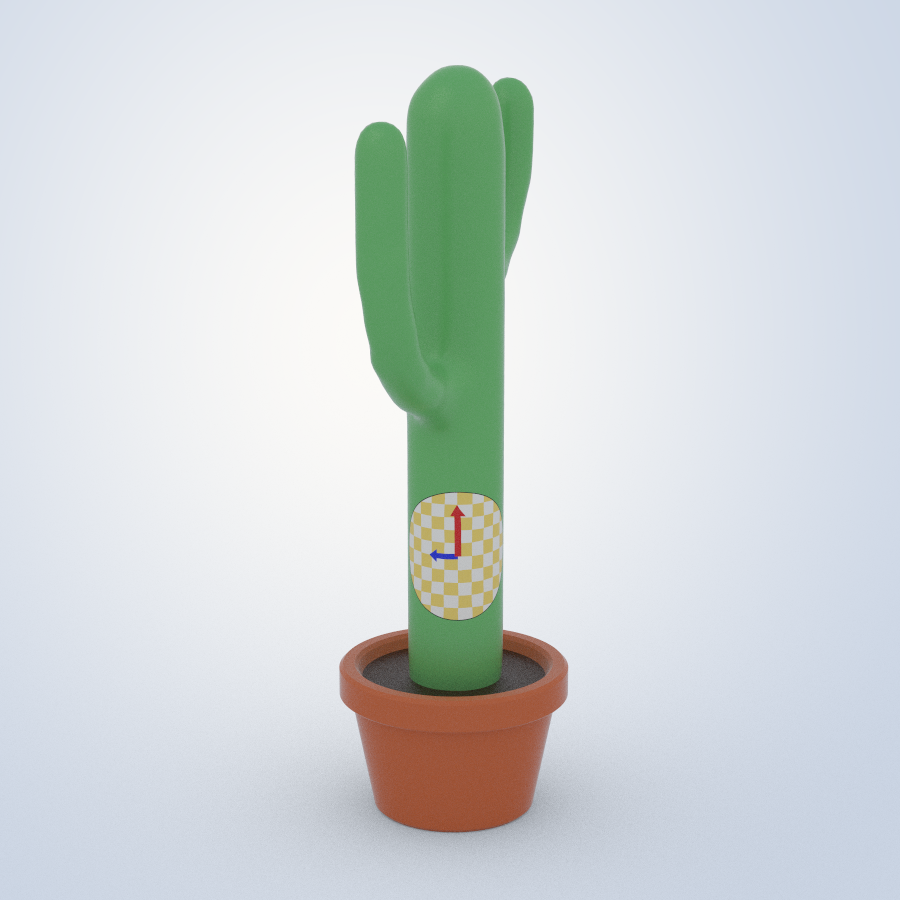
\includegraphics[width=0.42\linewidth]{../showcase/showcase_cactus.png}\hfill
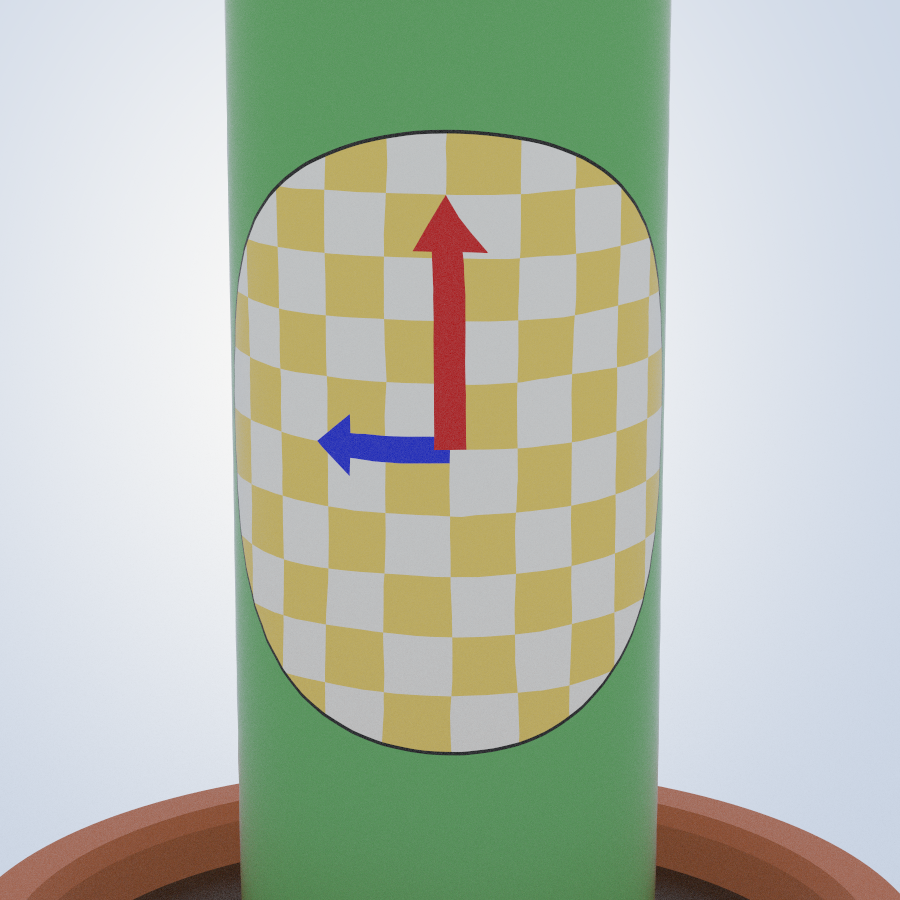
\includegraphics[width=0.42\linewidth]{../showcase/showcase_cactus_zoom.png}
\caption{A decal pasted with the logarithmic map, $(u, v) = r(\cos\theta, \sin\theta)$, with $r$ from the heat method and $\theta$ from the vector heat method with the intrinsic connection. The red arrow is the source direction, the blue one a quarter turn to its left.}
\label{fig:app_cactus}
\end{figure}

\paragraph{Why a smooth mesh.} On the coarse cactus of $502$ vertices used in the experiments, a few vertices are sharp cones, with angle defects up to $63.7^\circ$. A cone of positive defect $\kappa_v$ behaves like a small lens: the geodesics from $s$ that pass on either side of it are bent towards each other by the total angle $\kappa_v$, and behind the cone they cross. Points behind it are reached by two geodesics, and the exact logarithmic map folds over there: some triangles are mapped with the wrong orientation. We counted $29$ such flipped triangles inside a decal of radius $0.17$ on the coarse cactus refined by midpoint subdivision (which keeps the cones), against $2$ after Loop subdivision (which rounds them off). With the smooth cactus the largest defect is small, and the decal is clean. The renderer leaves untextured any face whose map is stretched more than four times in area, a sign of the cut locus:
\lstinputlisting[firstline=280, lastline=289, firstnumber=280]{../src/showcase.cpp}

\paragraph{The whole cactus.} Nothing stops us from using one logarithmic map for the whole surface: drop the radius of the decal and paint the checkerboard everywhere (Figure~\ref{fig:app_whole}, from a source on the front of the trunk). On the front, around the source, the squares are almost square, as in the decal. Away from it they shear and stretch, because the geodesics from $s$ spread apart around the trunk and are bent by the curvature of the arms. On the back, the geodesics that went around the trunk on the left meet those that went around on the right. That line is the cut locus: across it, $\theta$ jumps from about $+\pi$ to about $-\pi$, and the map is no longer one to one. The faces that straddle it are stretched past the guard and stay green, so the green seam down the back of the trunk is the cut locus, made visible by the method itself. One chart cannot cover a closed surface; a decal must stay on its own side of the cut locus.
\begin{figure}[t]
\centering
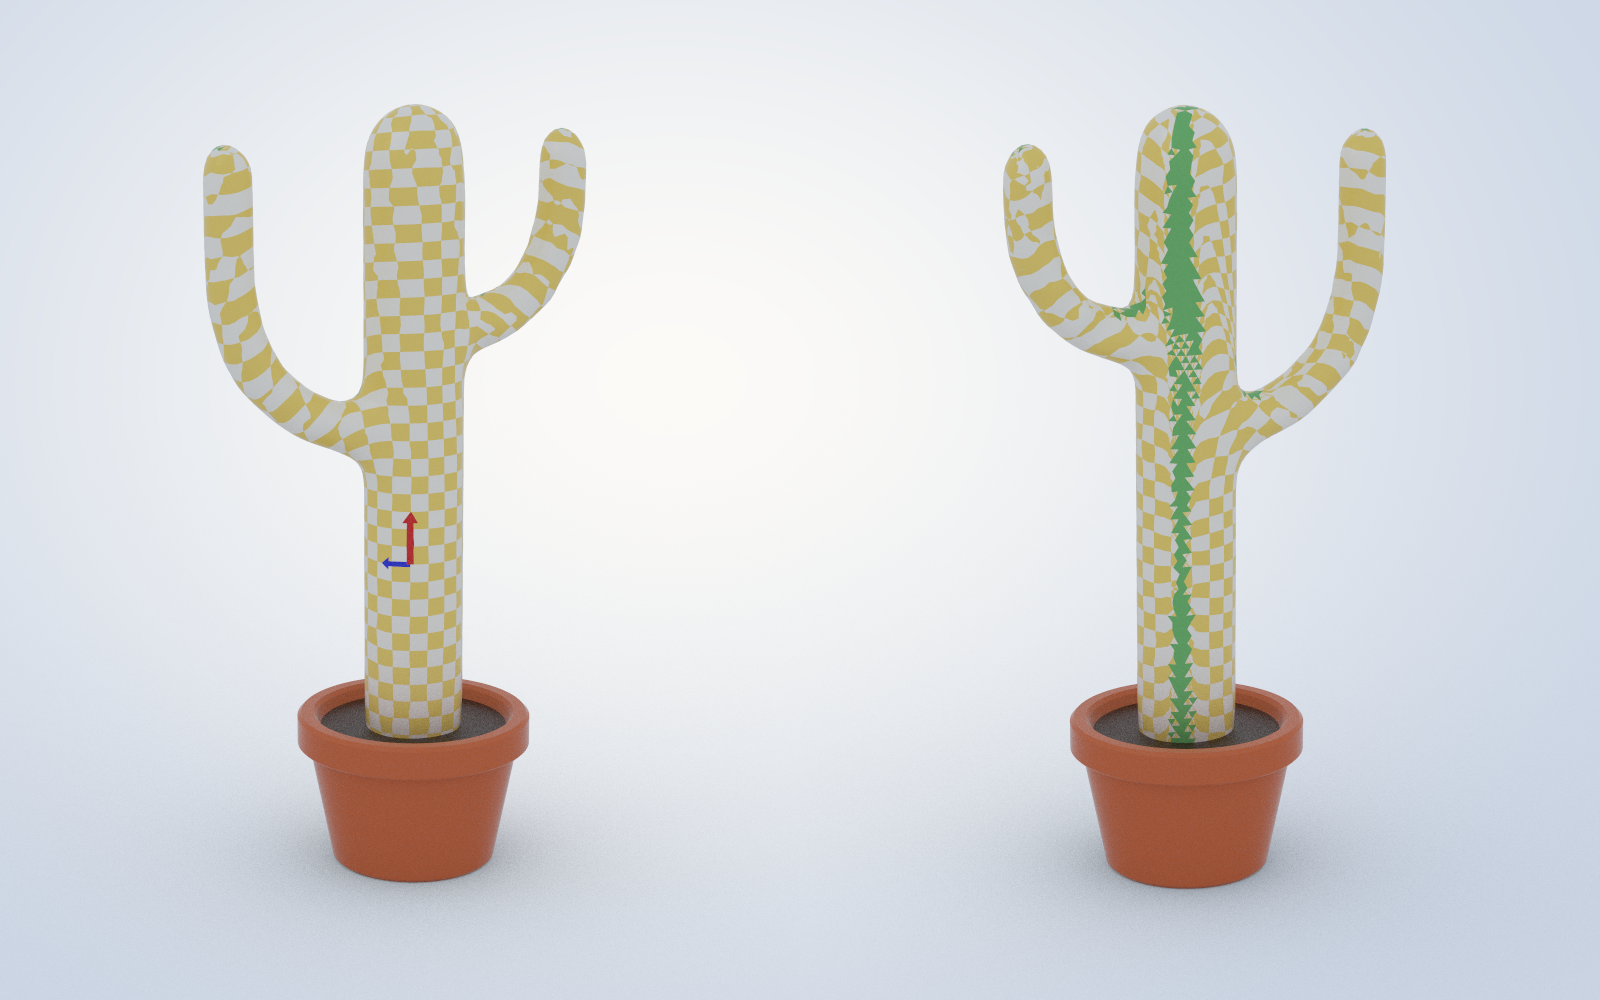
\includegraphics[width=\linewidth]{../showcase/showcase_whole.png}
\caption{One logarithmic map over the whole cactus. Left: the front, with the source and its two arrows. Right: the back; the green seam is the cut locus, where the geodesics that went around the two sides of the trunk meet and the map stops being one to one.}
\label{fig:app_whole}
\end{figure}

\paragraph{An atlas of charts.} The cure is the one of cartography: several charts, each used only near its own source. We take eight sources, one on the front and one on the back of the lower trunk, of the upper trunk and of each arm, compute the eight logarithmic maps, and give each point the chart of its geodesically nearest source. The boundary between the charts of two sources $s_1$ and $s_2$ is then the set of points equally far from both, $r_1 = r_2$; on a part shaped like a cylinder, with one source on each side, it runs along the sides of the part, a quarter turn from each source, while the cut locus of each chart is half a turn away, on the other side. So no chart is used up to its cut locus. Each chart is already turned upright (its red arrow along $e_z$), so two neighbouring checkerboards have nearly the same orientation; only their phases differ, and we remove the mean difference by translating each chart: on the vertices near the boundary with the charts placed before it, where $r_k$ is within three edge lengths of the nearest earlier $r_j$, we compute the mean of $\log_{s_j}(x_i) - \log_{s_k}(x_i)$ and add it to all the coordinates of chart $k$. The result is Figure~\ref{fig:app_atlas}: squares of nearly the same size everywhere, and boundaries that are visible only as small shifts of the pattern, mostly at the saddles where the arms meet the trunk. There the curvature is negative, and no flat chart, and no stitching, can keep every square a square.
\begin{figure}[t]
\centering
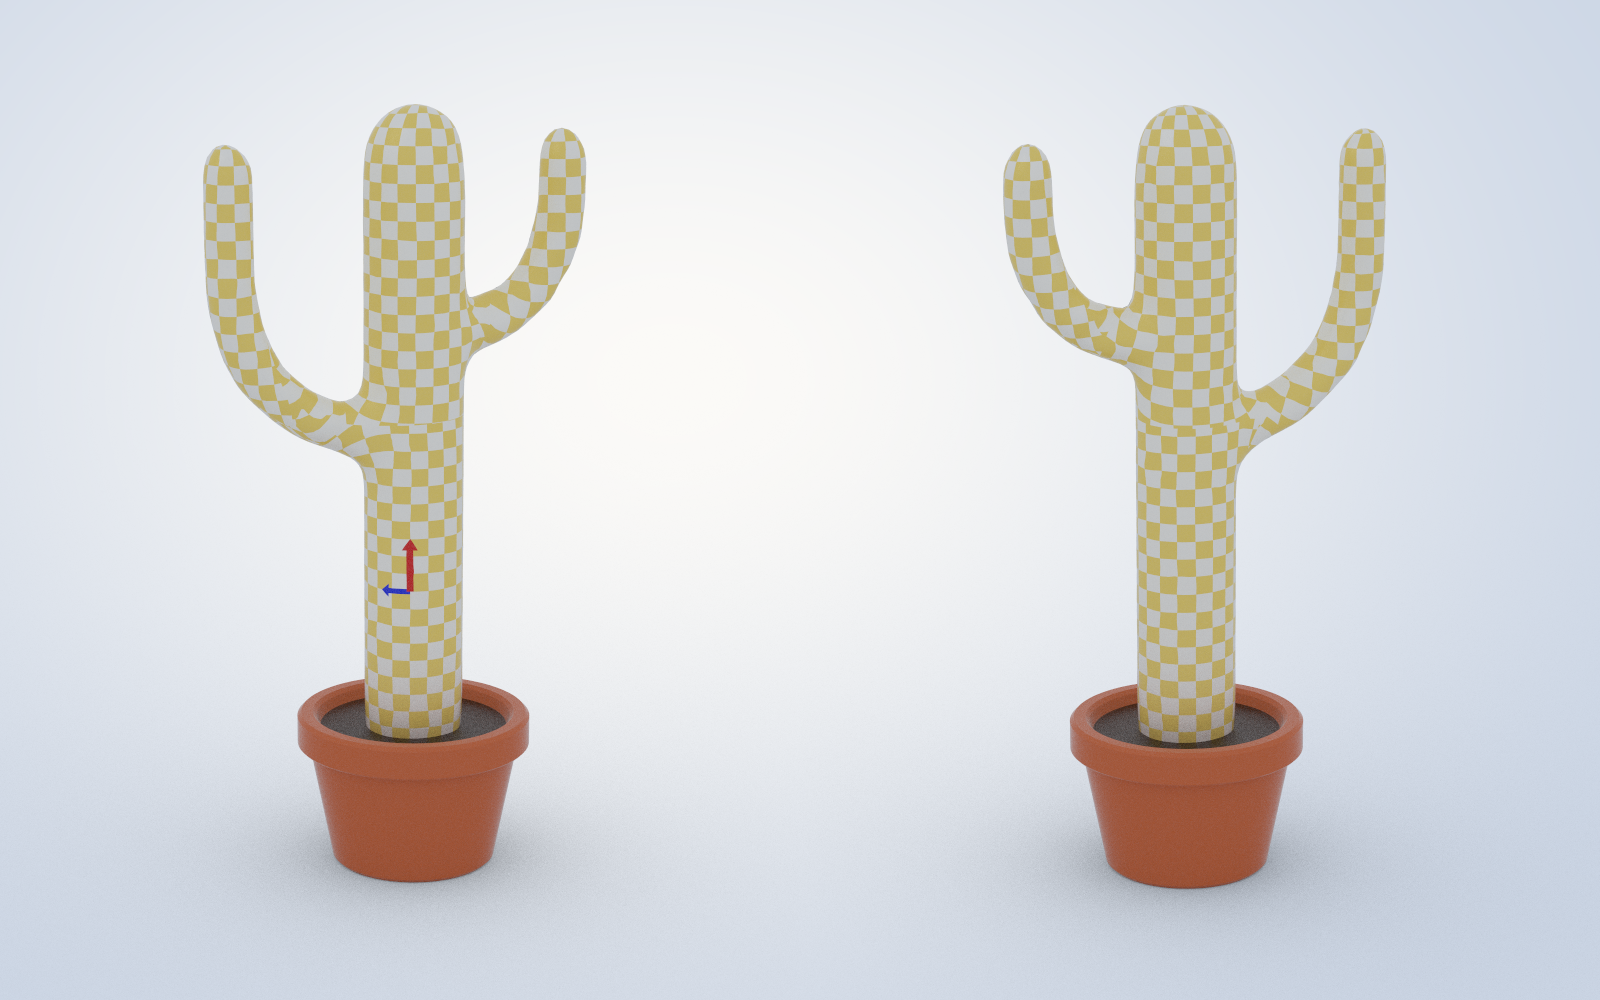
\includegraphics[width=\linewidth]{../showcase/showcase_atlas.png}
\caption{The checkerboard of Figure~\ref{fig:app_whole} with an atlas of eight logarithmic maps (front and back of the lower trunk, the upper trunk and each arm), each point painted by the chart of its nearest source, and the charts translated to match along their boundaries. The red and blue arrows mark the first chart.}
\label{fig:app_atlas}
\end{figure}

%%% ......................................................................
\subsection{Graph paper on the folded sheet: extrinsic against intrinsic}

The Miura-ori of Figure~\ref{fig:miura} is intrinsically flat, so its exact logarithmic map is simply its unfolding: lay the faces flat in the plane, one after another across their common edges, and read the plane coordinates relative to $s$. This gives us the exact $r$ and the exact $\nabla r$ in every face, so that we can compute the angle~(\ref{eqn:app_theta}) with the exact $R$ and isolate the only remaining ingredient, the transported direction $Y$, that is, the connection. The unfolding places the first face by its layout, and each next face by the rigid motion that puts its shared edge on the already placed one:
\lstinputlisting[firstline=166, lastline=205, firstnumber=166]{../src/showcase.cpp}
Line~196 finds the rotation angle $\gamma$ that turns the layout of $g$ so that its copy of the shared edge has the direction of the placed one; line~198 places the third vertex, and line~199 keeps $\gamma$. The angle $\gamma$ is kept for each face, because the exact $\nabla r$ in the face frame is the plane direction $p_i - p_s$ turned back by $-\gamma$.

We then compute the logarithmic map twice, with the corner connection of Part~\ref{part:ga} (rolling into the plane of the vertex normal) and with that of Part~\ref{part:intrinsic} (the bisector rule), and render graph paper with it (Figure~\ref{fig:app_miura}). If the map is exact, the lines of the paper are straight on the unfolded sheet, so on the folded sheet they run straight across every fold.
\begin{figure}[t]
\centering
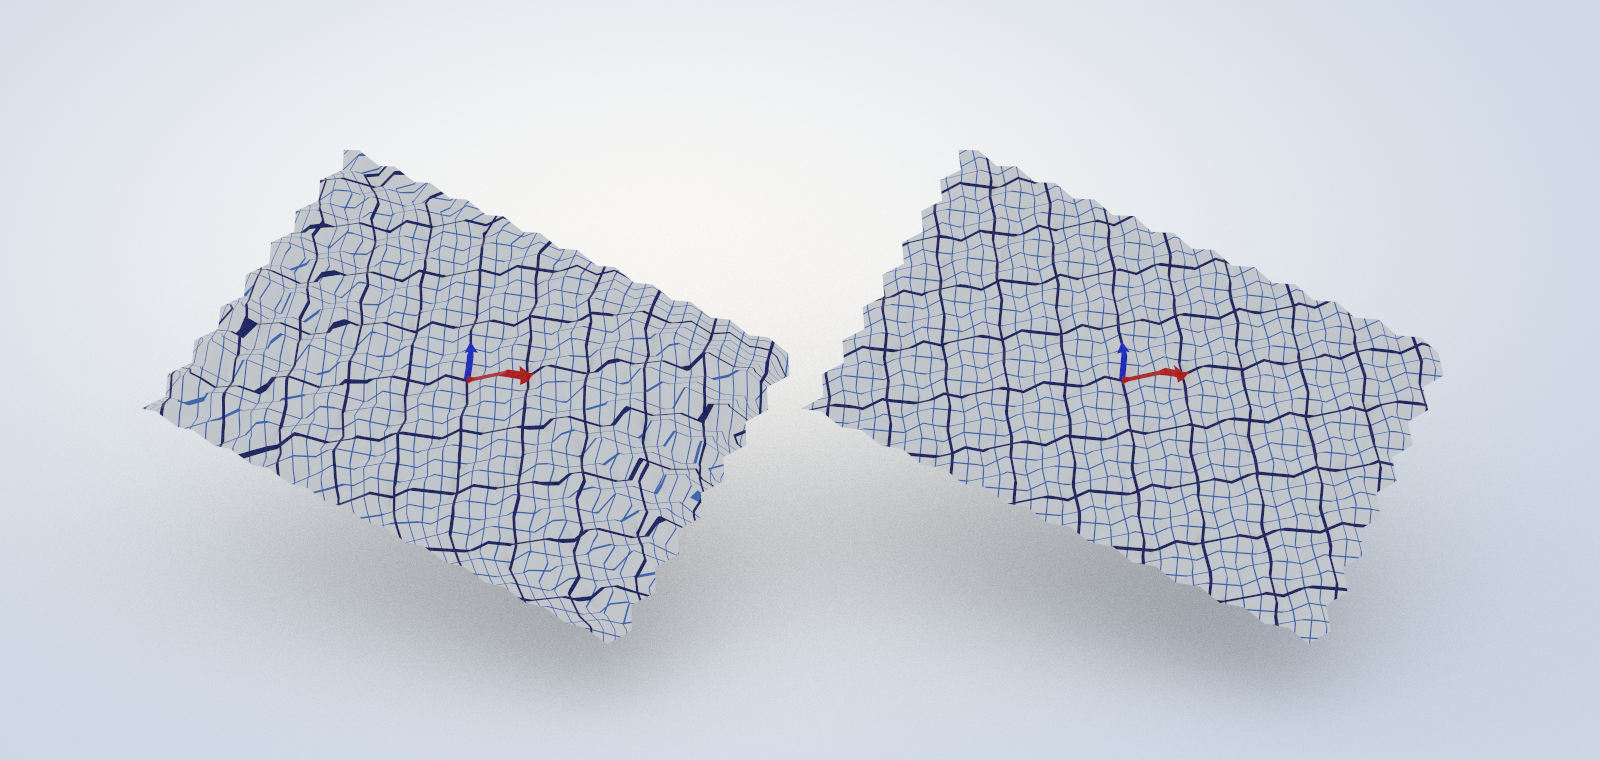
\includegraphics[width=0.95\linewidth]{../showcase/showcase_miura.png}
\caption{Graph paper on the folded Miura sheet, pasted with the logarithmic map from the center. Left: the extrinsic connection of Part~\ref{part:ga}; the lines break at the folds, and the angle is wrong by $2.2^\circ$ on average and up to $14.8^\circ$. Right: the intrinsic connection of Part~\ref{part:intrinsic}; the lines run straight across every fold, exactly as on the flat paper, with angle errors below $3\cdot 10^{-13}$ degrees.}
\label{fig:app_miura}
\end{figure}
The program measures, at every vertex, the angle between the computed coordinates and the exact unfolded ones:
\begin{center}
\footnotesize
\begin{tabular}{l c c}
\toprule
connection & mean angle error & largest angle error \\
\midrule
extrinsic, Part~\ref{part:ga} & $2.2^\circ$ & $14.8^\circ$ \\
intrinsic, Part~\ref{part:intrinsic} & $6.6\cdot 10^{-14}$ degrees & $2.7\cdot 10^{-13}$ degrees \\
\bottomrule
\end{tabular}
\end{center}
The intrinsic result is exact for the reason found in Section~\ref{section:int_connection}: at a flat vertex, $s_i = 1$, the bisector rule~(\ref{eqn:intrinsic_rho})~[\,$\rho_i^f = (\beta_e + \tfrac\alpha2) - s_i(\theta_e + \tfrac\alpha2)$\,] becomes $\rho_i^f = \beta_e - \theta_e$, which is the exact unfolding, so every transport the method makes is exact and so is $Y$. The extrinsic connection rolls the four faces of a Miura vertex into the plane of the vertex normal about four different axes; the rolled corners do not fit edge to edge, every transport is slightly wrong, and the errors add up along the paths from the source.

\paragraph{What the application shows.} The finite element machine of this text is reusable: the distance needed one more pass of the recipe, for scalars, with a variational problem (least squares for the gradient) instead of a heat step, and with one function-space subtlety (the constant in the kernel, fixed by $r(s) = 0$). And the difference between the two ways of giving a vertex a plane, which in the experiments of Section~\ref{section:int_experiments} was a column of small numbers, becomes something one can see.
